    %!TeX spellcheck = en-US
\documentclass[10pt, letterpaper]{article}
\usepackage[margin=1.3in,footskip=0.25in]{geometry}

\usepackage{yamauchi-template}
\usepackage{tabularx}


\newtheoremstyle{mytheoremstyle} % name
    {2\topsep}                    % Space above
    {2\topsep}                    % Space below
    {\itshape}                   % Body font
    {}                           % Indent amount
    {\bfseries}                   % Theorem head font
    {.}                          % Punctuation after theorem head
    {0.5em}                       % Space after theorem head
    {}  % Theorem head spec (can be left empty, meaning ‘normal’)


\theoremstyle{mytheoremstyle}

\newtheorem{question}{Question}[section]

\newcommand{\pr}[1]{\mathbb{\Pr}\left(#1\right)}
\newcommand{\E}[1]{\mathbb{E}\left[#1\right]}
\newcommand{\ind}[1]{\mathbf{1}\left(#1\right)}


\newcommand{\var}{\textnormal{Var}}
\newcommand{\cov}{\textnormal{Cov}} 
\newcommand{\cor}{\textnormal{Cor}} 

\usepackage{epigraph}
\usepackage{lipsum}


%% === abbs ===


\title{\textbf{Weighting in Modern Surveys}}
\author{\normalsize Shiro Kuriwaki\thanks{Postdoctoral Fellow. \href{https://www.shirokuriwaki.com}{\texttt{www.shirokuriwaki.com}}}}
\date{\normalsize POLISCI 450D ~~~ \today}



\begin{document}
\maketitle

\setstretch{1.2}

\epigraph{``Survey weighting is a mess.''}{Gelman (\href{http://www.stat.columbia.edu/~gelman/research/published/STS226.pdf}{2005}, \emph{Statistical Science})}


\section*{Motivation}

Most social science PhD students will use surveys for their own research. Modern surveys are increasingly cheap to collect, but perhaps increasingly unrepresentative. Therefore common challenges that students need to address with their survey data are often:

\begin{itemize}
\item ``Isn't your survey data unrepresentative of the population you care about?''
\item ``What happens to your findings among subset $S$ of your survey?''
\end{itemize}

\noindent Both questions require basic intuition about survey weights to answer. 




\section*{Illustrative Data (for Problem Set)}


\begin{minipage}{0.75\linewidth}
\hspace{1em}Since the 1950s, the German government conducts a 1\% sample of its residents. The U.S. Census Bureau also conducts a similar survey called the American Community Survey. Such surveys are the basis of many research articles, and the basis of even more government and private industry analytics. 

\vspace{0.1in}

\hspace{1em}Say we want to make inferences about Native Born Germans in former East Germany (GDR) states.  You run an online Qualtrics survey of this population. Because it is online, you have no control over any strata before running the survey. Rivers (\href{https://citeseerx.ist.psu.edu/viewdoc/download?doi=10.1.1.468.9645&rep=rep1&type=pdf}{2007}) was one of the first papers that showed how to match and re-weight such opt-in online surveys. 
\end{minipage} %
\begin{minipage}{0.25\linewidth}
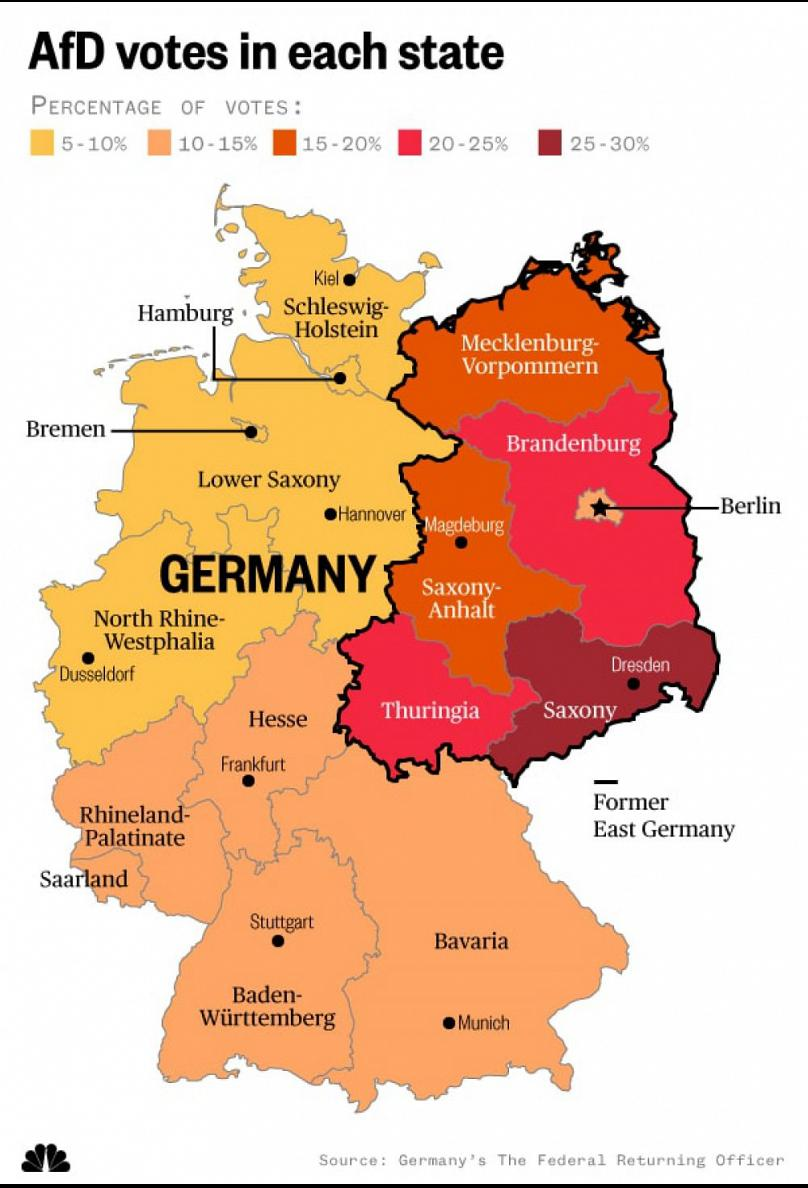
\includegraphics[width = \linewidth]{figs/afd-german-states.jpeg}
\end{minipage}

\vspace{0.2in}


In Canvas, download the rds file \texttt{samp\_GDR.rds}, which is a survey of $n =$ 1,000 of this population. It has the following variables:

\begin{itemize}
\item \texttt{Y} is a binary outcome variable of interest (e.g. Yes to some public opinion question). It is a synthetic variable I made up; the content is not important here. 
\item \texttt{educ} Education, which has three levels. ``Abitur'' are those who pass the final exam at the end of high school aiming for higher education (like the A-levels in the UK). ``Vocational'' are vocational schools in the former GDR. The rest are coded as ``No HighEd''. The dummy variables associated with this levels are \texttt{abitur} and \texttt{poly}.
\end{itemize}

Also download the rds file \texttt{pop\_GDR.rds} ($N=$ 100,000). This is the population this poll was sampled from, which is called a \textit{frame} in polling. In modern surveys, we do not have actual frames available, but we will use it here to explore the validity of weighting methods. 

\begin{itemize}
\item In this data, \texttt{D} is an indicator for Response / Selection / Survey Inclusion. It is recorded in the frame. It is 1 if the item in the frame ended up in the survey, 0 otherwise. 
\item Usually, the outcome \texttt{Y} is not in the population frame. (The whole point of a poll is that you can only observe the outcome you are interested in the sample). But we leave it in here for later validation.
\end{itemize}

(To avoid releasing proprietary data, this is quasi-synthetic of the actual data I obtained.)

\bigskip

The poll is a \emph{biased} sample of the population, so the goal is to make good (i.e. low bias, low variance) inferences about the population.  Load the data and answer the following questions.

\section{Post-stratification weighting}

The educational breakdown in the population and survey is as follows:

\bigskip

\begin{minipage}{0.5\linewidth}

\begin{center}
\textbf{Population}


\begin{tabular}[t]{lr}
\toprule
Education & Fraction\\
\midrule
Not High-Ed & 0.50\\
Abitur & 0.15\\
Vocational & 0.35\\
\bottomrule
\end{tabular}
\end{center}
\end{minipage} %
\begin{minipage}{0.25\linewidth}
\begin{center}
\textbf{Survey}

\begin{tabular}[t]{lr}
\toprule
Education & Fraction\\
\midrule
Not High-Ed & 0.33\\
Abitur & 0.25\\
Vocational & 0.42\\
\bottomrule
\end{tabular}
\end{center}
\end{minipage}


\begin{question}
What are post-stratification weights that will make the weighted proportion of the education in the survey equal to the target distribution in the population? 
\end{question}

It is often convenient to re-scale the weights by a scalar so that they are mean 1. We call this \textbf{normalized} weights $w_i$ for individual $i$. 

\begin{question}
What transformation would you apply to your weights to normalize them?  
\end{question}
\vspace{1in}

\begin{question}
Compute the sample proportion of $Y$, which we'll call $\widehat{\mu}$. How would you compute the weighted proportion in the sample with weights $w_i$? Is this weighted estimated guaranteed to be an unbiased estimator of the population mean of $Y$, which we'll call $\mu$?
\end{question}

Next, suppose we think that the outcome should vary by geography too. However, we are worried that the non-representativeness of the survey with respect to education will also show up within geographies.  You tabulate the data and find this frequency table. 

\begin{center}
\begin{minipage}{0.5\linewidth}
\singlespacing
\begin{tabular}[t]{llrr}
\toprule
State & Education & $n$ & frac\\
\midrule
Brandenburg & Not HighEd & 77 & 0.08\\
Brandenburg & Abitur & 45 & 0.04\\
Brandenburg & Vocational & 63 & 0.06\\
Mecklenburg-Vorpommern & Not HighEd & 51 & 0.05\\
Mecklenburg-Vorpommern & Abitur & 22 & 0.02\\
Mecklenburg-Vorpommern & Vocational & 51 & 0.05\\
Saxony & Not HighEd & 109 & 0.11\\
Saxony & Abitur & 93 & 0.09\\
Saxony & Vocational & 142 & 0.14\\
Saxony-Anhalt & Not HighEd & 58 & 0.06\\
Saxony-Anhalt & Abitur & 42 & 0.04\\
Saxony-Anhalt & Vocational & 86 & 0.09\\
Thuringia & Not HighEd & 70 & 0.07\\
Thuringia & Abitur & 25 & 0.03\\
Thuringia & Vocational & 66 & 0.07\\
\bottomrule
\end{tabular}
\end{minipage}
\end{center}

\begin{question}\label{ques:jointpost}
How would you post-stratify on both education and state? Verbally describe the procedure. You will implement it in R in the problem set. 
\end{question}

\begin{question}
Your friend is interested in another outcome. He takes the weighted mean of $Q$ with those weights. Does this estimator has the same guarantees of representativeness as $\widehat{\mu}_w$?
\end{question}

\begin{question}
Your friend is interested in estimating the average of $Y$ among non-married men in East Germany. She subsets the survey data to non-married men, takes the associated weights you computed, and produces weighted mean of the sample. What guarantees does this estimate  have?
\end{question}

In the rest of this document, we'll think about the limitations of this post-stratification weighting approach. That is, if you wanted to post-stratify on as many variables as possible, what new problems do you think this will create for you? All this will naturally motivate \emph{Multilevel Regression and} Poststratification (MRP), which we will discuss next week.

\section{Standard Errors}

\epigraph{``It is not always clear how to use weights in estimating anything more complicated than a simple mean or ratios, and standard errors are tricky even with simple weighted means.''}{Gelman (\href{http://www.stat.columbia.edu/~gelman/research/published/STS226.pdf}{2007})}

Weights are great at reducing bias but there is a bias-variance tradeoff. Let's first start with standard errors with no weights are no necessarily, i.e. when the sample is a SRS:

\begin{question}
Show that when the outcome of interest is binary, a simple random sample (SRS) of size $n$ has a (95\%) margin of error of roughly $1/\sqrt{n}.$ Interpret this quantity with proper units.
\end{question}
\vspace{0.5in}

Recall the standard error is the standard deviation of your estimator (i.e. the standard deviation of its sampling distribution). Standard Errors changes with weights. A classic formulation for computing standard errors with weights is the design effect formulation by Leslie Kish. 

With normalized weights $w_i$, the \textbf{design effect} in practice computed as
\begin{align}
\text{D}_{\text{eff}} = \frac{\frac{1}{n}\sum^n_{i=1}w_i^2}{(\frac{1}{n}\sum^n_{i=1}w_i)^2}
\end{align}

The definition of a design effect is the standard error of the weighted estimator relative to the standard error of the (unweighted) simple random sample version of that estimator.

\begin{question}
Show that $\text{D}_{\text{eff}}$ is a function of the variance of normalized weights. Is it an increasing or decreasing function of the variance of weights?
\end{question}

\vspace{0.5in}

Kish's \textbf{effective sample size} $n_{\text{eff}}$ is defined as the SRS sample size that would be needed to achieve the same variance as the weighted estimator.  Therefore, it can be computed as:

\begin{align}
n_{\text{eff}} = \frac{n}{\text{D}_{\text{eff}}}
\end{align}

\begin{question}
Show that the standard error of a weighted proportion $\widehat{\mu}_w$ is an increasing function of the variance in weights.
\end{question}

\vspace{0.1in}


This relationship between weights, variance, and effective sample size has clear implications for bias-variance tradeoffs and reducing total mean square error.



\section{The Balance Test Fallacy and Calibration Methods}

\epigraph{``Contrary to what is assumed by many theoretical statisticians, survey weights are not in general equal to inverse probabilities of selection''}{Gelman (\href{http://www.stat.columbia.edu/~gelman/research/published/STS226.pdf}{2007})}

\begin{question}
In the population frame, use the variable \texttt{D} (selection) to estimate the propensity score.  What is the Horvitz-Thompson weighted estimator?
\end{question}

Inverse probability weighting (IPW) works well in theory. Remember the propensity score theory (Rosenbaum and Rubin \href{https://academic.oup.com/biomet/article/70/1/41/240879}{1983}): If you control for the correct propensity score model in a biased sample, then your estimate of the population mean is unbiased (i.e., asymptotically). 

But propensity scores must be estimated from the data, and this is hard (Kang and Schafer \href{https://doi.org/10.1214/07-STS227
}{2007}). Thus the balance test is hard to get right, and is also misleading: aggressive weighting will lead to false negatives (Imai, King, and Stuart, \emph{JRSS A} \href{https://imai.fas.harvard.edu/research/files/matchse.pdf}{2008}). And small propensity scores ``explode'' the variance: a probability of 0.01 implies a weight of 100. The idea of \emph{calibration} is to avoid modeling the propensity score altogether, and instead just balance the covariates.


Imai and Ratkovic (\emph{JRSS B}, \href{https://imai.fas.harvard.edu/research/files/CBPS.pdf}{2014}) point out that a logit propensity score model's  MLE is identical to (``dual'' to) the covariate balancing constraint. That is, define  the propensity score model as a logit:

\begin{align}
\pi_\beta(X_i) = \frac{\exp{X_i^\prime\beta}}{1 + \exp{X_i^\prime\beta}}
\end{align}

The likelihood of all the data is the Bernoulli form

\begin{align}
\pi_\beta(X_i)^{D_i} (1 - \pi_\beta(X_i))^{1 - D_i}
\end{align}

for all observations $i$. To make things easier, as usual in MLE, we take the log:

\begin{align}
\sum_i D_i \log\{\pi_\beta(X_i)\} +  (1 - D_i)\log(1 - \pi_\beta(X_i))
\end{align}

To find the parameter $\beta$ that maximizes this likelihood (MLE), we solve for the score constraint: i.e. the first derivative of the log likelihood with respect to $\beta$.

\begin{question}
Show that the MLE of the propensity score model is identical to the covariate balancing condition.
\end{question}
\vspace{0.8in}

\begin{question}
Using the \texttt{CBPS} package (Imai et al.), compute Covariate Balancing Score Weights from the population and survey.
\end{question}

Hainmueller (\emph{Political Analysis}, 2012) formulated the entropy balancing score:

\begin{align}
\{w^{\texttt{ebal}}_i\}^N_{i=1} = \argmin_{w} \sum_{i: D_i = 0} w_i\log(w_i / w^{0}_i),\\
\text{subject to } \frac{1}{N}\sum_{i:  D_i=0}w_i f(X_i) =  \frac{1}{n}\sum_{i: D_i=1}w_i f(X_i)
\end{align}
where $w^{0}_i$ are merely base weights as starting values (e.g. all 1s), and $f(X_i)$ are various moments of the covariates (e.g. means). This also tries to finds low-variance weights that match a constraint. The idea derives from \textbf{rake weighting} in surveys:

\begin{quote}
 ``In particular, the [entropy balancing method] heavily borrows from the survey literature that contains several reweighting schemes which are used to adjust sampling weights so that sample totals match population totals known from auxiliary data (see Sarndal and Lundstrom 2006 for a recent review and earlier work by Deming and Stephan 1940, Ireland and Kullback 1968, Oh and Scheuren 1978, and Zaslavsky 1988 who proposed a similar log-linear reweighting scheme to adjust for undercount in census data).'' (Hainmueller 2012, p.27)
\end{quote}

\noindent Balancing weights are an active area of statistical research. See for example work by Zubizarreta et al. (\href{http://www.jrzubizarreta.com/minimal.pdf}{2017})

\begin{question}
Using the \texttt{ebal} package (Hainmueller), compute the same sort of weights with entropy balancing propensity scores.
\end{question}

\begin{question}
In Question \ref{ques:jointpost}, we presumed you had access to the joint distribution of state and education. Suppose that the German government does not give you that joint distribution, but it \emph{does} tell you the breakdown of education in all of the population and populations of each state. What can you do to try and post-stratify the data to the joint distribution of state and education? To validate your weights, you can use any number of raking functions in R: \texttt{survey::rake}, \texttt{iterake}, or \texttt{autumn}.
\end{question}

\end{document}
